\subsection{Problem Statement}

\subsubsection{Problem Context}
In software architecture, applications often manage elements stored across multiple disparate data structures. For example, a modern media streaming application may maintain an array-based queue for upcoming tracks, a doubly linked list for play history, and a binary search tree (BST) for genre organization.

Without an abstraction layer, the client application must implement specific traversal logic tailored to each container:
\begin{itemize}
    \item \textbf{Array / Contiguous Vector:} Relies on direct indexed access (\texttt{list[i]}).
    \item \textbf{Linked List:} Relies on node-by-node pointer traversal (\texttt{node->next} or \texttt{node->prev}).
    \item \textbf{Tree / Graph:} Requires recursive or stack-based traversal strategies (e.g., in-order, pre-order, DFS, or BFS).
\end{itemize}

\begin{figure}[H]
    \centering
    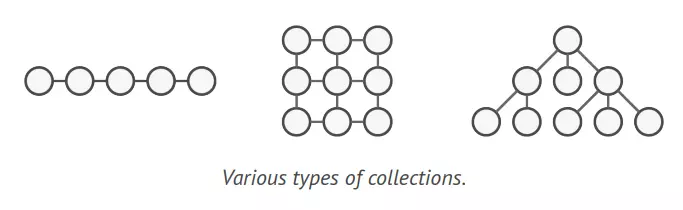
\includegraphics[width=0.7\linewidth]{Figures/desProblem.png}
    \caption{Problem of Direct Container Traversal~\cite{viblo_iterator}}
    \label{fig:iterator_problem}
\end{figure}

\noindent Exposing these low-level traversal mechanisms directly to consumer code introduces several architectural deficiencies and violates core object-oriented design principles~\cite{gof1994, refactoring_guru_iterator}:
\begin{itemize}
    \item \textbf{Encapsulation Leakage:} The internal structure, node pointers, and indexing models of the collection are exposed directly to the client.
    \item \textbf{Single Responsibility Principle (SRP) Violation:} The aggregate class is burdened with managing traversal state and access algorithms in addition to managing its core dataset.
    \item \textbf{Open/Closed Principle (OCP) Violation:} Introducing a new collection type or altering an existing data structure requires updating all client-side traversal loops across the codebase.
    \item \textbf{Code Duplication:} Traversal and rendering algorithms must be rewritten or overloaded for every individual container type.
\end{itemize}